\chapter{Context}
\label{chap:contexto}

\lettrine{I}{n} this section, we introduce the relevant context for this work that provides the basic concepts necessary for its understanding.
For this, we describe the field of ophthalmology and medical imaging, as well as the state of the art in image alignment.

\section{Ophthalmology}
\label{sec:Oftalmoloxía}
Ophthalmology is the medical specialty responsible for the study and treatment of eye diseases, including the eyeball, its musculature, the lacrimal system, and the eyelids.
The human eye is one of the organs we depend on most and provides the greatest amount of sensory information, as well as being one of the most complex in our body \cite{kanski2011clinical}.

The importance of ophthalmology lies not only in the treatment of eye diseases but also in its ability to provide valuable information about the patient's general health status.
Direct observation of blood vessels and neural tissue 'in vivo' allows ophthalmologists to detect early signs of various systemic diseases.
For example, glaucoma, which shows no symptoms in its initial stages, can be diagnosed through regular examinations of ocular pressure and the optic nerve \cite{importglaucoma}.
This early diagnostic capability makes ophthalmology a fundamental specialty in the prevention and maintenance of the patient's visual and general health.

\subsection{Anatomy of the human eye}
\label{subsec:Anatomía do ollo humano}
The eye is responsible for capturing light and transforming it into electrical impulses that are sent to the brain.
This information is interpreted by the brain, which through mechanisms such as attention and memory, enables visual perception. \cite{eyefunct}
The human eye is composed of several structures, each with a specific function that enables visual perception \cite{eyeanat}. Among them are:

\begin{itemize}
\item Cornea and Lens: work together to focus light on the retina. The cornea, located on the outside of the eye, provides most of the refractive power, while the lens, a flexible lens, adjusts focus for objects at different distances.
\item Pupil and Iris: regulate the amount of light entering the eye. The iris, the colored part of the eye, expands or contracts to control the size of the pupil, the central opening.
\item Retina: a layer of light-sensitive cells (photoreceptors) that convert light stimuli into electrical signals, initially processed in the retina itself.
\item Optic nerve: carries electrical signals generated in the retina to the brain, where they are interpreted as images.
\item Optic disc: also known as the "blind spot," is the area where the optic nerve exits the eye; it lacks photoreceptors.
\item Blood vessels: distribute necessary nutrients and oxygen to the retina and remove its metabolic waste.
\end{itemize}

Figure \ref{fig:imaxes_ojo} shows these structures located in images.

\begin{figure}[tbp]
    \centering
    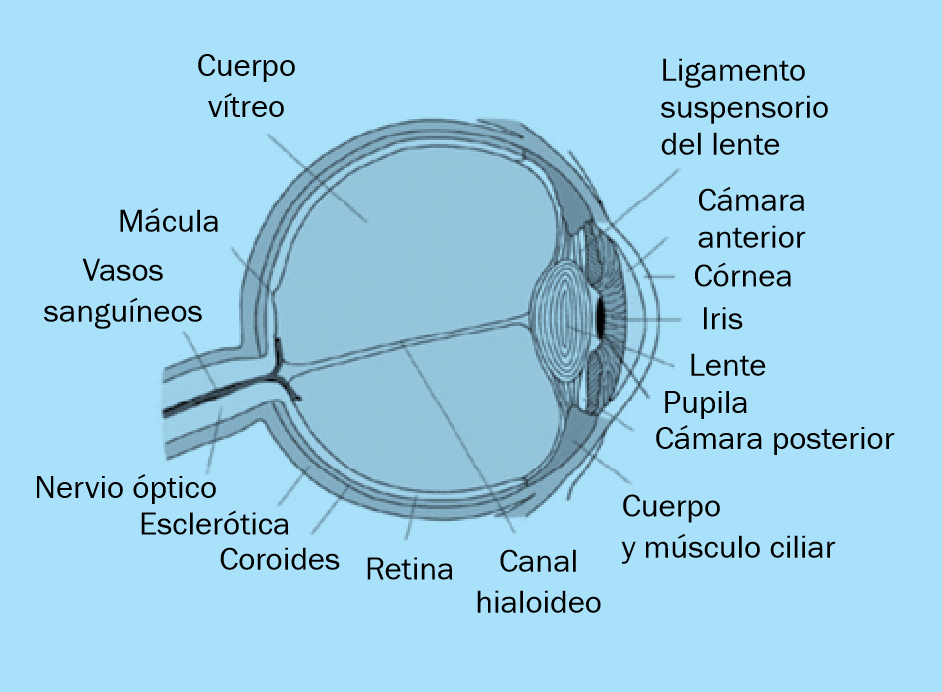
\includegraphics[width=0.45\textwidth]{imaxes/ojo1.png}
    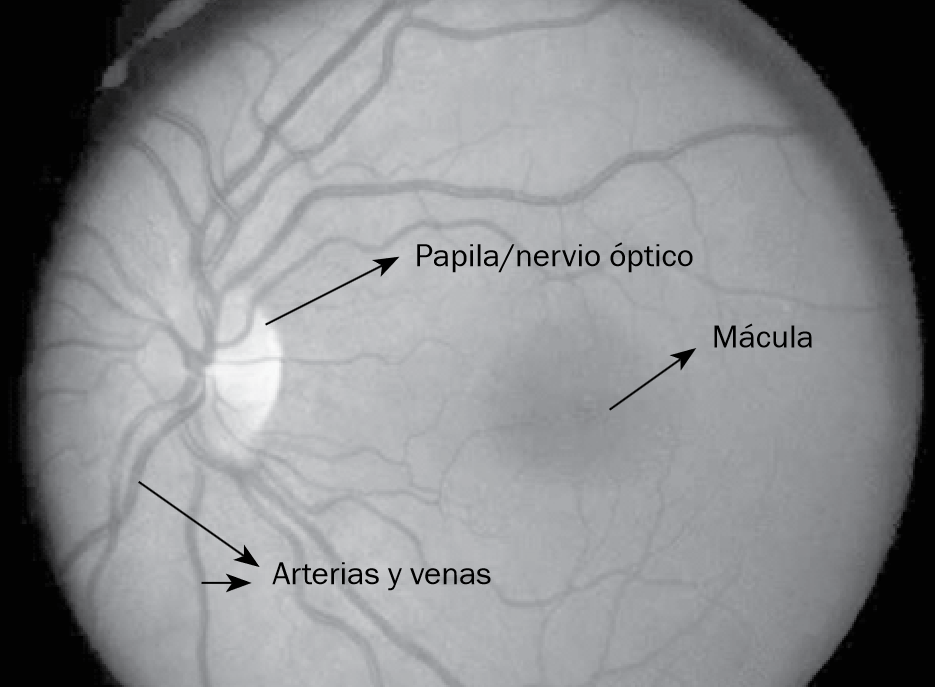
\includegraphics[width=0.45\textwidth]{imaxes/ojo2.png}
    \caption{Images of the human eye, taken from \cite{visionyojo}. On the left, annotated lateral view of the eye. On the right, annotated retinography of the eye.}
    \label{fig:imaxes_ojo}
\end{figure}

\subsection{Ophthalmic Imaging}
\label{subsec:Imaxe oftalmolóxica}
There are various medical imaging modalities that allow observation of the eye, each with different properties and applications.
These include fundus photography, optical coherence tomography (OCT), and fluorescein angiography \cite{ilginis2014ophthalmic}.

This work focuses on fundus photography among other reasons due to its common use in clinical practice.
This is largely due to its accessibility, requiring cheaper equipment and less training compared to other modalities.
Additionally, it is a non-invasive and quick technique to perform, making it preferable in most cases \cite{retinimaging}.

It is performed using a special camera called a retinograph, and generally requires prior dilation of the patient's pupil.
This allows more light to enter the eyes, which leads to better visualization of the retina and improves image quality.
A specialist can analyze the retinography to detect signs of diseases such as diabetic retinopathy, hypertension, or macular degeneration \cite{retreggood}.

\section{Image Registration}
\label{sec:Rexistro de imaxes}
Image registration is a process that consists of, with two or more images, determining the spatial correspondence between them
and aligning them in a common coordinate system, with the objective that the features of interest are found in the same position.

Image registration has utility in many different fields such as satellite imaging, geography, robotics... but the
field of medical imaging is one of the most interesting for its practical application and is the one addressed in this work \cite{goshtasby2017theory}.
These images can vary temporally, spatially, dimensionally, or in modality.

In healthcare, proper registration can be used to compare images of the same patient taken at different times, in different modalities, or to compare between different patients.
This allows reviewing the progress of a disease over time, fusion of images from different modalities, or detection of common patterns between different individuals.
Image fusion allows much better interpretation of the available information in them and is of great help in guiding doctors in decision-making.
It is also useful for correcting involuntary patient movements during image acquisition, such as in the case of breathing in lung images, or for image-guided radiation therapy (\gls{IGRT}) which
could not function without the proper use of image registration techniques \cite{wang2022neuralrenderingstereo3d}.

Until recently, much of the registration work was done manually by experts with software like BigWarp \cite{bigwarp},
and depended on the professional's skills to detect features of interest and perform alignment.
This made the process slow and error-prone, as well as impractical for large volumes of images.

Figure \ref{fig:retin_reg} shows an example of retinal image registration, where you can observe how the images are aligned so that anatomical structures coincide.

\begin{figure}[tbp]
    \centering
    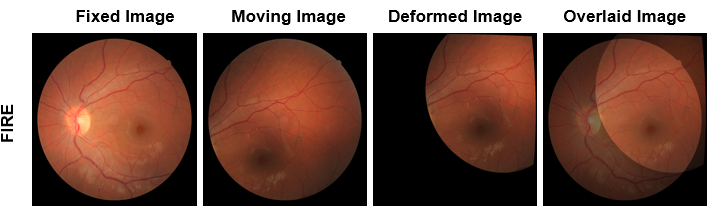
\includegraphics[width=0.8\textwidth]{imaxes/retin-reg.png}
    \caption{Example of retinal image registration \cite{sivaraman2024retinaregnetzeroshotapproachretinal}}
    \label{fig:retin_reg}
\end{figure}

\subsection{Registration Categories}\label{subsec:Registration categories}

Image registration can be classified into different categories according to their characteristics.

\begin{itemize}
    \item \textbf{According to number of images:}
    \begin{itemize}
        \item \textit{Pairwise:} Registration is performed between two images, one fixed and one moving.
        \item \textit{Multiple:} Several images are registered simultaneously, seeking global correspondence.
    \end{itemize}

    \item \textbf{According to modality:}
    \begin{itemize}
        \item \textit{Intra-modality:} Images belong to the same modality (for example, two retinographies).
        \item \textit{Inter-modality:} Images come from different modalities (for example, retinography and OCT).
    \end{itemize}

    \item \textbf{According to transformation type:}
    \begin{itemize}
        \item \textit{Rigid:} Only allows translation and rotation, maintaining distances and angles.
        \item \textit{Affine:} In addition to translation and rotation, allows scaling and shearing.
        \item \textit{Deformable (non-rigid):} Allows complex local and non-linear deformations.
        \item \textit{Diffeomorphic:} Non-rigid transformation that is continuous, invertible and differentiable throughout its domain. Without this characteristic, the transformation cannot be guaranteed to be reversible, which is why they are preferred in many cases \cite{han2022diffeomorphicimageregistrationneural}.
    \end{itemize}

    \item \textbf{According to automation level:} \cite{deeplernreview3dreg}
    \begin{itemize}
        \item \textit{Manual:} The user selects control points or adjusts parameters.
        \item \textit{Automatic:} The process is performed without human intervention, using algorithms.
        \item \textit{Semi-automatic:} Combines manual and automatic intervention.
    \end{itemize}

    \item \textbf{According to transformation nature:}
    \begin{itemize}
        \item \textit{Symmetric:} The transformation is consistent in both directions between images.
        \item \textit{Asymmetric:} The transformation is calculated in only one direction. When working with images asymmetrically, the reference image is called the fixed image and the image to be registered is called the moving image.
    \end{itemize}

\end{itemize}

Global linear transformations are usually represented in transformation matrices, where each matrix element represents a transformation parameter.

For more complex transformations, deformation vector fields (\gls{DFV}s) are used, which allow representing local deformations in the image, making it much more flexible to represent non-linear and detailed transformations.
DFVs are typically represented with a matrix of the same size as the image, where each element represents a vector indicating the direction and magnitude of the deformation.

This work is situated in pairwise, intra-modality image registration with deformable transformations. It is a fully automatic process that produces asymmetric transformations.

Figure \ref{fig:dfv_visualization} shows two ways to visualize a DFV: using arrows that indicate the direction and magnitude of deformation, and applying the deformation to a grid to see how it distorts.

\begin{figure}[tbp]
    \centering
    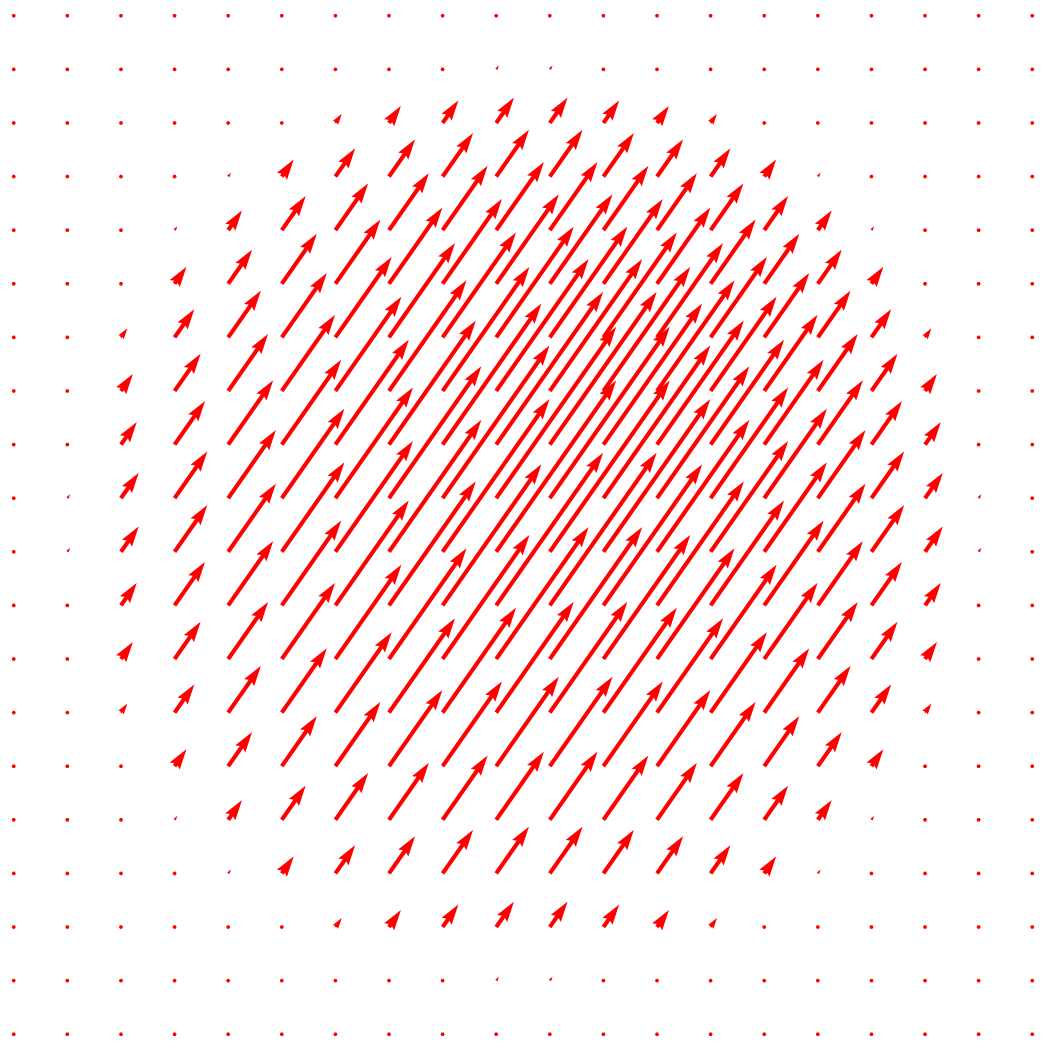
\includegraphics[width=0.45\textwidth]{imaxes/dfv_arrows.png}
    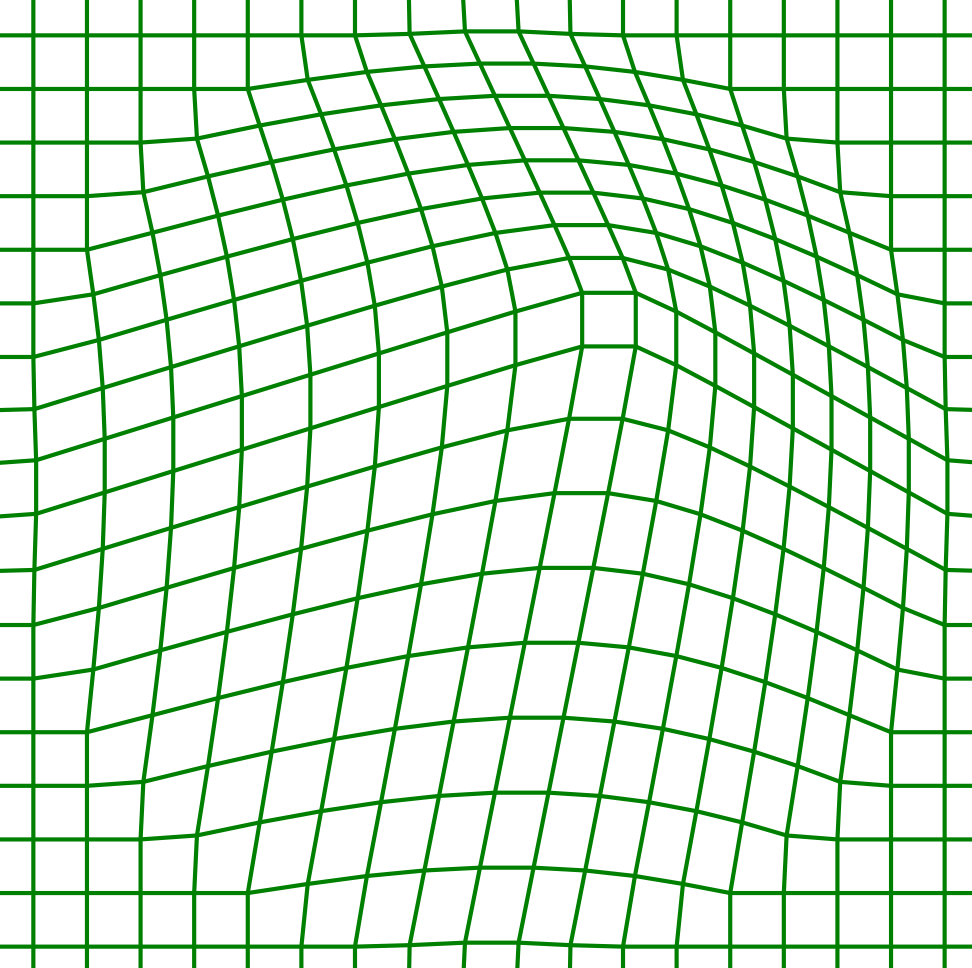
\includegraphics[width=0.45\textwidth]{imaxes/dfv_grid.png}
    \caption{Visualization of the deformation vector field (DFV). On the left, arrow representation. On the right, this deformation applied to a grid.}
    \label{fig:dfv_visualization}
\end{figure}

\subsection{State of the art}
\label{subsec:State of the art}

Medical image registration constitutes a fundamental research area that has experienced important advances in recent decades. In this field, registration accuracy and robustness are especially relevant, as they are used for disease diagnosis and monitoring, as well as for surgical treatment planning.
In the field of ophthalmology, methods that work well in various medical imaging domains (brain, lungs, etc.) often require adjustments to work on retinas, so there is a parallel state of the art.

The evolution of registration methods in retinographies reflects the transition from purely algorithmic approaches to hybrid methodologies, where recent publications like HybridRetina \cite{liu2024progressiveretinalimageregistration} show how combining both approaches is beneficial to achieve the best results, taking advantage of the precision of classical methods and the adaptability of machine learning methods.

\subsubsection{Classical methods}\label{subsubsec:Métodos clásicos}

Classical medical image registration methods can be classified into two main categories:
Those based on image similarity (\gls{IBR}) and those based on features (\gls{FBR}).
There are also hybrid methods that combine both approaches \cite{integrateintfeat}.
The final result can be the transformation parameters or the fused image.

\paragraph{Image similarity-based methods}
\label{par:Métodos baseados en similitude de imaxe}

Registration is performed by comparing pixel or voxel intensity values using a similarity metric between the fixed image and the moving image.
This approach tends to require multiple iterations to converge, in which the degree of similarity between images is calculated and
transformation parameters are updated using an optimization mechanism until termination criteria are met.

Traditional registration methods have three main components: the similarity metric, the optimizer and the transformation model.

Figure \ref{fig:rexistro_iterativo} shows a diagram of the iterative registration process.

\paragraph{Feature-based methods}
\label{par:Métodos baseados en características}

Registration is performed by identifying and matching salient features between images, such as points, lines or edges.
Typically, these methods have 3 main steps:

\begin{itemize}
\item \textbf{Interest point detection:} Identification of salient points or regions in images, such as edges, corners or textures. Algorithms like SIFT \cite{sift}, SURF \cite{surf}, BRISK \cite{brisk} or FREAK \cite{freakkeypoint} can be used for this.
\item \textbf{Feature description:} detected points are described and compared between images using descriptors.
\item \textbf{Transformation estimation:} once correspondences are found, the transformation that aligns the images is calculated using matching algorithms like FLANN \cite{flann} or RANSAC \cite{ransac}.
\end{itemize}

Some of the traditionally most used methods in this field are \gls{GDB-ICP} \cite{GDB-ICP} and Harris-PIIFD \cite{piifd}. The latter uses the Harris algorithm \cite{Harris1988ACC} for interest point detection, describes them with \gls{PIIFD}, and matches them using \gls{BBF} \cite{BBF}.
Finally, matches are refined and the transformation (rigid, affine or polynomial) is chosen according to the number of valid point pairs. Several improvements have been proposed on this basis to adapt it to multimodal retinal registration such as UR-SIFT \cite{ur-sift} or \gls{GMM} \cite{GMM}.

An advantage of this approach is the ability to register images with large local variations or different modalities, as it does not depend as much on global image similarity.

Other relevant classical methods in the field of eye imaging include REMPE \cite{rempe}, which simultaneously estimates camera pose and eye shape. It uses an ellipsoidal model for the eye and estimates camera positions with RANSAC, then refines it with a PSO variant \cite{pso}.

\begin{figure}[tbp]
\centering
\begin{tikzpicture}[node distance=2cm, scale=0.8, every node/.style={transform shape}]
% Nodes
\node (imageFixa) [process] {Fixed Image};
\node (imageMobil) [process, right of=imageFixa, xshift=3cm] {Moving Image};
\node (featureExtraction) [process, below of=imageFixa, yshift=-1cm] {Similarity Measure Calculation};
\node (parameterUpdate) [process, below of=featureExtraction, yshift=-1cm] {Parameter Update};
\node (applyTransformation) [process, below of=parameterUpdate, yshift=-1cm] {Apply Transformation};
\node (criteriaCheck) [decision, below of=applyTransformation, yshift=-1cm] {Criteria Met?};
\node (result) [process, below of=criteriaCheck, yshift=-1cm] {Result};
% Arrows
\draw [arrow] (imageFixa) -- (featureExtraction);
\draw [arrow] (imageMobil) -- (featureExtraction);
\draw [arrow] (featureExtraction) -- (parameterUpdate);
\draw [arrow] (parameterUpdate) -- (applyTransformation);
\draw [arrow] (applyTransformation) -- (criteriaCheck);
\draw [arrow] (criteriaCheck) -- node[anchor=west] {Yes} (result);
\draw [arrow] (criteriaCheck.east) -- ++(1,0) node[anchor=south, xshift=0.5cm] {No} |- (featureExtraction.east);
\end{tikzpicture}
\caption{Iterative image registration process}
\label{fig:rexistro_iterativo}
\end{figure}

There are also multiple programs that use these methods in tools to facilitate image registration, such as SimpleITK \cite{simpleitk}, Elastix \cite{elastix} or ANTs \cite{ants}.

\subsubsection{Deep learning methods}\label{subsubsec:Deep learning methods}

With the arrival of deep learning methods to medical imaging, neural networks began to be used for image alignment.
There is great interest in deep learning-based methods, as reflected in the growing number of publications in the field. Figure \ref{fig:method_comp} shows the evolution of the number of publications on image registration, differentiating between deep learning-based methods and traditional methods.

Deep learning methods can be classified into two types depending on whether annotated \glossary{DFV}s are required or not in the training stage:
supervised (require annotations) and unsupervised (do not require annotations) \cite{nie2024medicalimageregistrationapplication}.

According to the degree of supervision used in the training stage, supervised methods can be divided into fully supervised or weakly supervised.
Fully supervised registration uses reference DVFs to supervise the learning process, and the loss term is usually based on the discrepancy between reference DVFs and predicted DVFs.

Weakly supervised registration can use other implicit reference labels, not based on explicit data like DVFs, but rather using indirect information to guide the registration process, such as image similarity or constraints based on anatomical structure shapes or boundaries.
More than two types of reference data are frequently used to train weakly supervised registration models \cite{bharati2022deeplearningmedicalimage}.

Unsupervised methods have the advantage of not requiring annotated data, which is a great advantage since one of the biggest challenges for medical image networks is collecting quality training data \cite{medicalimageanalysis}.
Creating annotated DVF datasets is a laborious and costly process that normally can only be executed by specialists, which is why unsupervised registration methods are of great interest.
Similar to iterative methods, it is common to use a similarity metric between images along with a regularization term to guide the optimization process avoiding falling into unrealistic transformations.

Deep learning approaches are useful both in their ability to learn the registration task end-to-end, and to replace specific modules of the traditional process.
In this sense, deep learning methods can be categorized according to which registration process task they replace.

\begin{figure}[tbp]
\centering
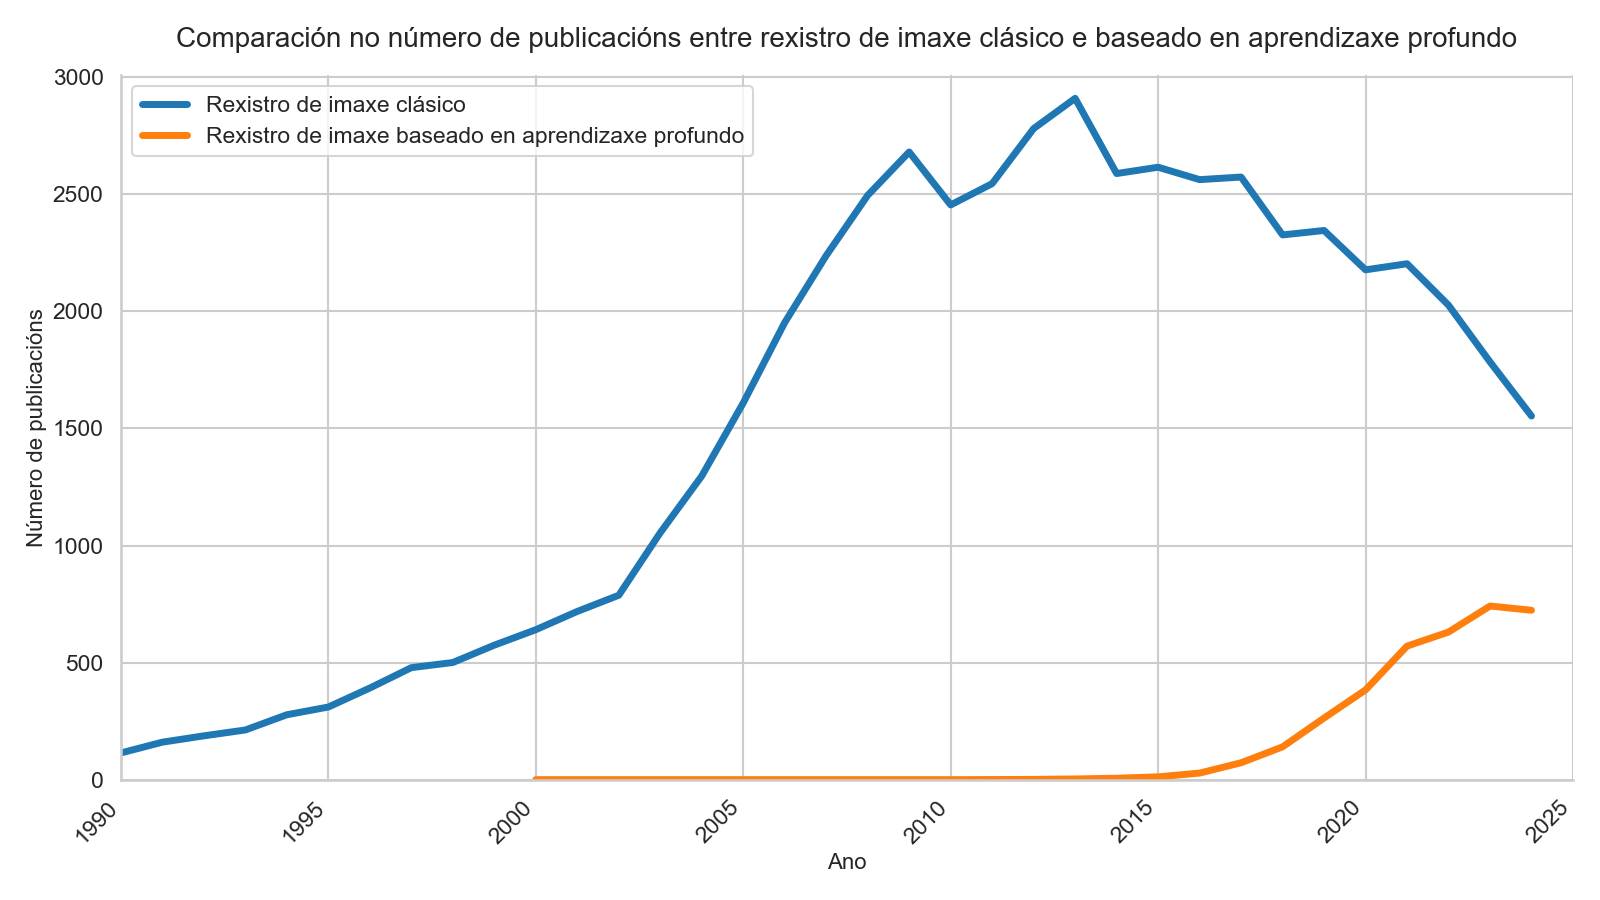
\includegraphics[width=0.8\textwidth]{imaxes/methods_comp.png}
\caption{Comparison of publications over time related to image registration. Data extracted from Scopus \cite{scopus}, performing the queries: "TITLE-ABS-KEY(image AND registration) AND NOT(deep AND learning)" and "TITLE-ABS-KEY(image AND registration) AND (deep AND learning)"}
\label{fig:method_comp}
\end{figure}

Deep learning methods can replace any of these steps that make up classical registration methods independently or in combination.

\paragraph{In intensity-based registration (IBR)}
\label{par:IBR_substitution}

\begin{itemize}
\item \textbf{Similarity metric:} Deep learning methods can learn more robust similarity metrics than traditional ones. These learned metrics can be more effective in multimodal images or with artifacts.
For example, Czolbe et al. \cite{semanticsimilarity} propose two semantic similarity metrics that learn image similarity by comparing extracted high-level features. They present an unsupervised approach using autoencoders and a semi-supervised one that incorporates segmentation data.
\item \textbf{Optimizer:} Deep learning methods can replace the traditional iterative optimization process with networks that learn to directly predict optimal transformation parameters. A common approach is to use these datasets to optimize a CNN that, given two new unseen images, predicts the corresponding DVF \cite{defregcnn}. During the training process, the network can have access to DVFs with the correct deformation, or they can be obtained indirectly through optimization of an image similarity metric.
\item \textbf{Transformation model:} These methods learn implicit representations of the transformation through neural networks, allowing modeling of more complex deformations than traditional parametric models. Methods like IDIR \cite{wolterink2021implicit} fit into this category, using implicit neural fields to represent registration transformations.
\end{itemize}

\paragraph{In feature-based registration (FBR)}
\label{par:FBR_substitution}

\begin{itemize}
\item \textbf{Feature detectors:} Neural networks can learn to detect more robust and repeatable interest points than classical detectors like \glossary{SIFT}. SuperPoint \cite{superpoint} introduces a neural network-based feature detector that learns to detect and describe interest points simultaneously.
\item \textbf{Feature descriptors:} Descriptors learned through neural networks can capture more discriminative information, improving subsequent matching accuracy. These methods learn representations that are invariant to domain-specific transformations.
\item \textbf{Matching:} Neural networks can learn to perform robust feature matching, especially in the presence of illumination or perspective changes. SuperGlue \cite{superglue} is an example of a model that learns to match detected interest points using an attention-based architecture to capture relationships between points.
\end{itemize}

\paragraph{Direct regression methods}
\label{par:direct_regression}

Deep learning tends to require a large amount of data for training, which can be a disadvantage since in many cases annotated databases of the necessary size are not available.

Direct regression methods learn to map directly from a pair of images to transformation parameters, without the need for iterative optimization or explicit feature extraction.

They are also called amortized inference methods due to their ability to perform multiple inferences (registrations) after a single training process, as opposed to traditional methods that require individual optimization for each pair of images.
These approaches are useful for their computational efficiency in the inference phase. Voxelmorph \cite{Balakrishnan_2019voxelmorph} is one of the most used frameworks in deformable image registration, using models based on \gls{CNN}s and also allowing incorporation of auxiliary information (such as segmentations) if available, thus improving registration accuracy.

Methods like UDIR-Net \cite{undefreg} or DIO \cite{Jena_2025} also implement these ideas.

\subsubsection{State of the art in retinography registration}\label{subsubsec:Estado_da_arte_no_rexistro_de_retinografías}

Retinal image registration presents a unique set of challenges that distinguish it from other medical imaging domains.
One of the main obstacles are non-rigid deformations. These deformations can originate from the projection of the curved 3D retinal surface onto a 2D image or variations in the eye shape of each patient. Additionally, it is common to find image pairs with minimal overlap areas which makes it difficult to identify correspondences for alignment. This is compounded by variations in illumination, contrast and color between images captured in different situations, as well as anatomical changes induced by pathologies, which alter the structures used for registration.
Finally, the scarcity of public datasets, especially for specific conditions or populations, represents a significant barrier for developing supervised learning models.

The difficulty in obtaining reference deformation fields for training has driven the development of unsupervised frameworks. These models are trained by optimizing a loss function based on image similarity between the deformed moving image and the fixed image, along with a regularization term on the smoothness of the deformation.

Within classical methods, feature-based registration (FBR) approaches continue to be references in terms of accuracy. Among them, VOTUS \cite{Votus} stands out, being especially robust with low-overlap images and representing vascular trees as graphs to find correspondence between them. REMPE \cite{rempe} is another previously mentioned method in this category.

In the deep learning field, RetinaRegNet \cite{sivaraman2024retinaregnetzeroshotapproachretinal} is a recent zero-shot model that uses features extracted from diffusion models to establish correspondences, achieving state-of-the-art results.

ConKeD (Contrastive Keypoint Descriptors) and its evolution, ConKeD++, focus on perfecting the creation of keypoint descriptors, one of the most critical components of feature-based methods (FBR).
The main advantage is that it obtains results comparable to state-of-the-art classical methods (like REMPE and VOTUS) but with much faster execution times.

Most of these algorithms are evaluated and compared using the FIRE \cite{FIRE} reference dataset, allowing objective performance quantification.

\section{Neural Implicit Representations}
\label{sec:Representación Neuronais Implícitas}

Knowledge representation is one of the most important problems in computing, and deep networks are one of the most useful tools, especially in computer vision.
Traditionally, discrete representations are used, where the input space is divided into cells and each cell is assigned a value (for example point clouds, pixel matrices or voxels...).
One of the main disadvantages of these representations is that their complexity increases rapidly with the number of dimensions represented, in addition to the associated memory cost.

Neural implicit representations are an innovative paradigm that allows modeling continuous signals through functions parameterized by neural networks.
They encode information as a continuous function, which maps input values to corresponding output values, instead of directly storing feature values or signals.

Representing the signal as a continuous function allows solving problems associated with discretization and obtains other advantages.

INRs are much more efficient due to the implicit compression of information they perform. At the same time, it allows a level of detail not limited by image resolution, but by the network's capacity.
Additionally, continuous representations are differentiable, which allows gradient and derivative calculations analytically instead of having to approximate them through finite differences.
This also means that implicit representations are resolution-independent, allowing reconstruction at any spatial scale.

Typically, an MLP is used as architecture to represent the implicit function. However, using the ReLU activation function tends not to obtain the best results, as they are unable to represent local deformations without affecting their global behavior \cite{rahaman2019spectralbiasneuralnetworks},
so much research is directed at finding alternatives that improve signal representation. \cite{essakine2024standimplicitneuralrepresentations}

One of these alternatives is SIREN \cite{sitzmann2020implicitneuralrepresentationsperiodic}, which we will explore in more detail later.
Other proposals include \cite{ramasinghe2022periodicityunifyingframeworkactivations} which proposes Gaussian activation functions as an alternative to SIREN, and argues they can obtain better and more robust representations.
\cite{saragadam2023wirewaveletimplicitneural} provides a new wavelet-based activation function, which seems to be especially useful for image representation.

Implicit representations can be classified into two categories: generalizable and overfitted \cite{yu2024neuraltrajectorymodelimplicit}.
Overfitted representations focus on accurately reproducing a single signal, while generalizable representations can model several in the same network.

\subsection{Applications}
\label{subsec:Aplicacións}

INRs are used in all types of fields, from image generation \cite{reddy2022multiimplicitneuralrepresentationfonts}, through
object reconstruction \cite{mildenhall2020nerfrepresentingscenesneural} \cite{mescheder2019occupancynetworkslearning3d} or complex signal modeling \cite{wu2021iremhighresolutionmagneticresonance}.

Implicit representations are receiving increasing attention from the medical community, and are
especially useful for inverse imaging tasks, which require reconstructing correct representations from incomplete or noisy data \cite{molaei2023implicitneuralrepresentationmedical}.
Methods like NeRP proposed using implicit representations for reconstructing magnetic resonance images from incomplete data,
and obtained results comparable to traditional methods \cite{shen2023nerpimplicitneuralrepresentation}.

NeRF uses implicit representations to synthesize new viewpoints in 3D scenes \cite{mildenhall2020nerfrepresentingscenesneural},
optimizing a continuous volumetric function that models volume density and emitted radiance at each point in space.
They use an MLP, whose input is a single continuous 5D coordinate (spatial location (x, y, z) and viewing direction (θ, φ))
and whose output is the volume density and view-dependent emitted radiance at that spatial location.
The only input needed to optimize their representation is a set of images with known camera poses.
This work demonstrates that implicit representations are capable of modeling complex 3D scenes with high visual fidelity.

Implicit representations also have considerable potential in trajectory planning,
where INRs are used to model environments and plan trajectories for one or multiple agents \cite{yu2024neuraltrajectorymodelimplicit}.
The main advantage of doing it this way versus the traditional way (computationally intensive algorithms, especially for multi-agents) is the speed at which they find solutions (below millisecond on GPUs).
The biggest disadvantage is that they don't guarantee convergence to an optimal collision-free solution, but the authors demonstrate that the quality of generated trajectories is adequate for most applications \cite{trajectinr}.

In the medical field, these types of representations are used to ensure patient safety during teleoperated surgery and optimize robot trajectory to avoid collisions with the patient, for example in the mouth and throat \cite{teleoperatdrob}.
With this method, mesh reconstruction from images is avoided, which is a costly and imperfect process, and it is modeled using an INR from available medical data.
The operator's hand movement commands are taken as input by the model, which after an optimization process, generates a collision-free movement sequence that will be sent to the robotic hand.
They are also used to create 3D reconstructions of lungs that mitigate distortions caused by respiratory motion \cite{velikova2024implicitneuralrepresentationsbreathingcompensated}.

Another interesting use of neural implicit representations is image compression. Algorithms like COIN \cite{coin} represent input data using implicit neural networks (functions that map coordinates to RGB values), achieving efficient compression and significant reduction in encoding time across many modalities.

\subsection{Registration based on Neural Implicit Representations}\label{subsec:Rexistro_baseado_en_INRs}

Image registration based on Implicit Neural Representations (INR) parameterizes the deformation transformation as a continuous function, usually with a Multilayer Perceptron (MLP), which maps spatial coordinates to displacement vectors. Unlike CNNs, the network does not process image intensities directly, but is optimized using these to calculate the loss. One of the advantages in this context is the ability to calculate exact analytical gradients of the transformation, allowing more precise regularization than with approximations from grid-based methods.

Periodic activation functions (SIREN \cite{sitzmann2020implicitneuralrepresentationsperiodic}) allowed overcoming the problem of low-frequency transformation biases of the MLP, and were used by IDIR achieving state-of-the-art results \cite{wolterink2021implicit}.

The main drawbacks are slow inference (requires optimization for each pair of images) and the tendency to generate spatial foldings (unrealistic deformations). Current research focuses on hybrid models to mitigate these problems.
Some of the most relevant approaches include:
SINR (Spline-enhanced INR) combines INR with B-splines, where the network predicts displacements of a sparse control grid. This imposes smoothness intrinsically and facilitates multimodal registration \cite{SINR}.
Cycle-consistent INRs, which simultaneously train the forward and inverse transformation, using each network as a regularizer for the other to improve robustness.
Meta-learning: Learns an optimal weight initialization from a large dataset to drastically accelerate convergence during inference \cite{learnedinit}.
Geometry-conditioned INRs: Incorporate prior anatomical knowledge to simplify the complexity of the deformation to be learned \cite{harten2023deformable}.
Sun et al. \cite{sun2024medicalimageregistrationneural} propose an image registration that uses neural fields to model the transformation, also using positional encoding (which transforms spatial coordinates into high-dimensional vectors) allowing the network to more easily learn high-frequency transformations.

The use of Implicit Neural Representations (INR) for image registration offers remarkable precision by modeling deformation as a continuous and analytically differentiable function. This approach, exemplified by IDIR's initial success, allows more exact regularization than grid-based methods. However, its practical application is hindered by slow optimization for each image pair and the risk of producing unrealistic deformations with spatial foldings. The current state of the art tends to address these challenges through hybridization.

\section{Proposed work}
\label{sec:Traballo proposto}

The proposed work is situated within deep learning methods, and more specifically in intensity-based registration (IBR) using implicit neural representations (INRs).

As we have shown in this chapter, despite the potential of implicit neural representations in various medical domains, their specific application to retinal image registration remains unexplored.

This lack of research is especially relevant given the potential advantages offered by INRs, such as the ability to model complex deformations and their resolution independence.

Based on the framework introduced by \cite{wolterink2021implicit}, it is proposed to modify it to adapt it to the task of retinal image registration. The objective is to achieve consistently accurate registrations, especially in the FIRE dataset containing real retinal images.

This adaptation represents a novel contribution to the state of the art in retinal image registration, exploring for the first time the potential of implicit neural representations in this specific domain.